\documentclass{beamer}
\usepackage{tikz}
\usetheme{Antibes}

\begin{document}


\title[]{Diffusion Models for Tissues and Tumor Growth}
\author[Daniel Henricks]{Daniel Henricks
  \date{March 20th, 2024}
}


\begin{frame}
  \maketitle
\end{frame}
\begin{frame}
  \frametitle{Introduction}
  \begin{itemize}
    \item Researchers have studied cancer and tumor growth patterns for thousands of years
    \item First models: described tumors based on color and sensitivity to touch.
    \item Application of mathematical models to tumor growth gained traction in the 20th century
    \item Paper discusses an overview of two influential diffusion papers: Hill (1928) and Greenspan (1972)
  \end{itemize}
\end{frame}

\begin{frame}
  \frametitle{Hill's Paper on Diffusion}
  \begin{itemize}
    \item Discussed the diffusion constant, $k$. This constant is usually very small when discussing processes in the body.
    \item Modeled diffusion of oxygen and lactic acid through tissues. Conclusion: Not all oxygen can be absorbed.
    \item Derived equations for steady-state diffusion of oxygen and lactic acid
  \end{itemize}
\end{frame}

\begin{frame}
  \frametitle{Diffusion of Oxygen Within a Steady State}
  \begin{itemize}
    \item Fick's first and second laws of diffusion (next slide)
    \item Derived differential equation for oxygen concentration, $y$
    \item Maximum absorption of oxygen in a tissue of thickness $x'$
  \end{itemize}
\end{frame}

\begin{frame}{Fick's First and Second Laws of Diffusion}
  First law:
  \begin{equation}
    J = -k \frac{dy}{dx}
  \end{equation}
  J = the rate of diffusion (diffusion flux), k = diffusion rate (also known of diffusivity), $\frac{dy}{dx}$ = concentration gradient.
  \begin{itemize}
    \item Particles move from high to low concentration.
  \end{itemize}
  Second law:
  \begin{equation}
    \frac{dJ}{dx} = k\nabla^2J
  \end{equation}
  \begin{itemize}
    \item If one dimension, can simplify Laplacian
  \end{itemize}
\end{frame}

\begin{frame}{Deriving Oxygen Concentration}
  Using Fick's second law (one dimension, assumption of constant concentration):
  \begin{equation}
    \underset{\text{Usage Rate}}{\underbrace{a}} = k \frac{d^2y}{dx^2}
  \end{equation}
  Solution: 
  \begin{equation}
    y = \frac{ax^2}{2k} + bx + y_0
  \end{equation}
  After finding $b$ and maximum penetration distance, we get 
  \begin{equation}
    Y = \int_{0}^{\sqrt{\frac{2ky_0}{a}}} \frac{ax^2}{2k} + bx + y_0 dx = y_0 \frac{x'}{3}
  \end{equation}
  \begin{itemize}
    \item Conclusion: Not all oxygen absorbed by tissue
  \end{itemize}
\end{frame}

\begin{frame}
  \frametitle{Combining Oxygen and Lactic Acid Diffusion}
  \begin{itemize}
    \item Combining 2 diffusion equations in the same tissue
    \item Modeled the interaction of oxygen and lactic acid in a muscle
    \item Derived the ratio of oxygen consumed to lactic acid removed: $\frac{a}{\alpha}$
  \end{itemize}
    
  \begin{figure}[h!]
    \centering
    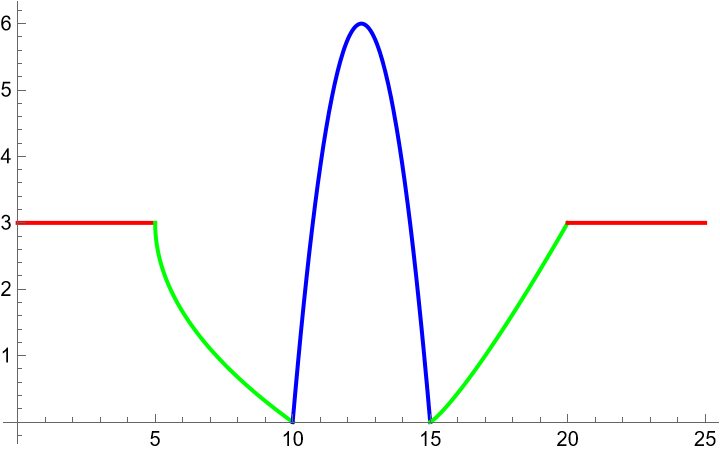
\includegraphics[width=0.5\textwidth]{graphics/image.png}
    \caption{Red: Steady state condition $y_0$. Green: $y$ decreases as you go further into the tissue. Blue: $y'$, lactic acid increases towards center of tissue.}
    \label{fig:image}
  \end{figure}

\end{frame}

\begin{frame}
  \frametitle{Greenspan's Paper: Models for the Growth of a Solid Tumor by Diffusion}
  \begin{itemize}
    \item Aimed to find what changes the outer radius of the tumor. Proposition: chemical substance.
    \item Modeled the tumor as a sphere with a necrotic core, middle layer, and outer layer
    \item Utilized the same diffusion model as Hill (1928); referenced Burton (1966), a famous paper on diffusion with tumors. 
  \end{itemize}
\end{frame}

\begin{frame}
  \frametitle{Illustration of a Tumor Model}
  \begin{figure}[ht]
    \centering
    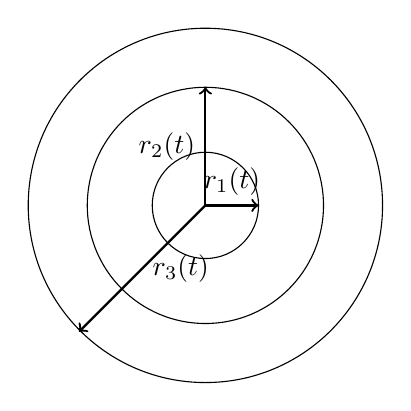
\begin{tikzpicture}[scale=1.5]
        \draw (0, 0) circle (1.5);
        \draw (0, 0) circle (1);
        \draw (0, 0) circle (0.45);

        \draw[->, thick] (0, 0) -- (0.45, 0) node[midway, above] {$r_1(t)$};
        \draw[->, thick] (0, 0) -- (0, 1) node[midway, left] {$r_2(t)$};
        \draw[->, thick] (0, 0) -- (-1.07, -1.07) node[midway, right] {$r_3(t)$};
    \end{tikzpicture}
    \caption{A cross-section of the sphere that represents the tumor. The necrotic core is situated between $0 < r < r_1$,
        the middle layer is situated between $r_1 < r < r_2$, and the healthy outer layer is located between $r_2 < r < r_3$.}
    \label{fig:cross-section}
\end{figure}

\end{frame}


\begin{frame}
  \frametitle{Conservation of Mass and Volume Equation}
  \begin{itemize}
    \item Derived the conservation of volume equation (3.1 in Greenspan) 
    \begin{equation}
      r_3^3(t) = r_3^3(0) + 3\int_{0}^{t} dt \int_{\max(r_1(t), r_2(t))}^{r_3(t)} S(\sigma, \beta) r^2 dr
      - \int_{0}^{t}3\lambda r_1^3(t) dt
  \end{equation}
    \item Modeled the inward movement of live tumor cells towards the necrotic center (push volume towards center)
    \item Time partial derivative: how tumor grows with time
  \end{itemize}
\end{frame}

\begin{frame}
  \frametitle{Diffusion Equations for Tumor Growth}
  \begin{itemize}
    \item Derived diffusion equations for $\beta$ (inhibitor) and $\sigma$ (nutrients) using Fick's second law
    \item Diffusion equations for each of these two derived:
  \end{itemize}
  \begin{equation}
    \frac{1}{r^2} \frac{\partial}{\partial r} r^2 \frac{\partial}{\partial r} \beta(r, t) = \frac{-P}{k'}
  \end{equation}
  \begin{equation}
    \frac{1}{r^2} \frac{\partial}{\partial r} r^2 \frac{\partial}{\partial r} \sigma(r, t) = \frac{a}{k}
\end{equation}
\end{frame}

\begin{frame}
  \frametitle{Solving the Diffusion Equations}
  \begin{itemize}
    \item Solving the equations directly turns out to be very hard
    \item Assuming $r$ is in the correct region, many simplifications can be applied.
    \item Verified the solutions, which are: 
  \end{itemize}
  \begin{equation}
    \beta = \frac{Pr_1^3}{3k'}(\frac{1}{r} - \frac{1}{r_3})
  \end{equation}
  \begin{equation}
    \sigma = [\sigma_{\infty} - \frac{a}{6k}(r_3^2 - r^2) + \frac{ar_1^3}{3k} (\frac{1}{r} - \frac{1}{r_3})]
\end{equation}
\end{frame}

\begin{frame}
  \frametitle{Present day models}
  \begin{itemize}
    \item Diffusion is applied to model many common problems (biology, emissions, air pollution)
    \item A recent paper by Stepien et al. (2015) included a diffusion model for in vitro glioblastoma growth:
  \end{itemize}
  \begin{equation}
    \frac{\partial u_i(r, t)}{\partial t} = \underset{\text{Diffusion}}{\underbrace{k \nabla^2 u_i}} + \underset{\text{Logistic growth}}{\underbrace{g u_i \left(1 - \frac{u_i}{u_{\max}}\right)}} - \underset{\text{Taxis}}{\underbrace{\nu_i \nabla_r \cdot u_i}} + \underset{\text{Shed cells from core}}{\underbrace{s \delta(r - R(t))}}
  \end{equation}

\end{frame}


\begin{frame}
  \frametitle{Conclusion}
  \begin{itemize}
    \item Hill and Greenspan proposed similar diffusion models for their respective problems
    \item Many modern diffusion models build upon these foundational works
    \item Diffusion models are versatile and somewhat simple to work with
  \end{itemize}

  Thanks!
\end{frame}

\end{document}